\documentclass{ti2}

% Dateikodierung ist utf8
\usepackage[utf8]{inputenc} 
\usepackage{listings}

\newcommand{\mm}{\emph}  

\begin{document}

% Nr, Abgabedatum, Gruppenleiter, Gruppenname, Name1...Name4
\Abgabeblatt{4}{28.11.2016}{Marc Hildebrandt}{C/06}%
                {Niklas Koenen}{Jan Klüver}%
                {Vincent Jankovic}{}%

\section*{Aufgabe 1} Zuerst erkälren wir unseren Code der Shell und dann kommt ein kleiner Testbericht.
\subsection*{Code:}
Nachdem der schon vorhandene Code durchlaufen wurde (eine if-Abfrage f"ur \mm{exit} wurde noch von uns hinzugef"ugt, denn dieser Befehl muss manuell angelegt werden), erzeugen wir einen Kindprozess mit \emph{fork()}. \emph{fork()} liefert uns die Adresse des Kindprozesses. Konnte der Elternprozess  auf Grund eines Fehlers nicht dupliziert werden, gibt \emph{fork()} eine $-1$ zurück. Diesen Fall fangen wir mit einer Fehlermeldung ab. Konnte der Kindprozess erzeugt werden, liefert \mm{fork()} dem Kindprozess eine 0. Ist dies der Fall, wird der eingegebene \mm{command} und die Paramerter mit der Envoirmentvariable \mm{getenv("PATH")} am Doppelpunkt getrennt und in \mm{sub} gespeichert. Vorher legen wir noch eine \mm{bool} Variable an, die uns sp"ater Hilft, die Erzeugung eines neuen Prozesses zu "uberpr"ufen. Nach der Zerlegung wird mit einer \mm{while}-Schleife jedes command (bzw. der Pfad) durchgegangen und umgewandelt. Zudem wird eine \mm{stat}-Variable angelegt, die den \mm{PATH} "uberpr"uft. Existiert der Pfad, so wird ein Prozess erzeugt und der command ausgef"uhrt (mit \mm{execv(s, cmd.argv)}). Danach sammeln wir alle Kindprozesse "uber den Signalhandler ein und benutzen \mm{wait(0)}, um die Terminierung zu erkennen. Dann kann ein neuer Befehl eingegeben werden.

\begin{lstlisting}
#include <stddef.h>
...

#include "parser.h"

using namespace std;

int main()
{
    for (;;)
      {
	struct command cmd = read_command_line();
	
	if(strcmp(cmd.argv[0], "exit") ==0)
	  {
	     exit(EXIT_SUCCESS);
	  }
	
	cout << "command: " << cmd.argv[0]
	     << ", background: " << (cmd.background ? "ja" : "nein") << endl;
	cout << endl;
	/* Hier muesste die Ausfuehrung stehen */
	
	pid_t pid;
	int status=0;
	bool neuerPro = false;
	
	pid=fork();
	
	if(pid == -1)
	  {
	    perror("Fehler!");
	  }
	else if (pid == 0)
	  {
	    char* command = getenv("PATH");
	    char* sub = strtok (command, ":");
	    while(sub != NULL)
	      {
		char s[200]= "";
		strcpy(s,sub);
		strcat(s,"/");
		strcat(s, cmd.argv[0]);
	        struct stat st;
		if( stat(s, &st) == 0)
		  {
		    neuerPro = true;
		    execv(s, cmd.argv);
		  }
		sub = strtok (NULL, ":");
	      }
	    if(!neuerPro)
	      {
		cout << "Sorry aber der Befehl ist Muell!!" << endl;
	      }
	    exit(EXIT_FAILURE);
	  }
	else
	  {
	    pid=wait(&status);
	    while(!WIFEXITED(status) && !WIFSIGNALED(status))
	      {
		pid=wait(0);
	      }
	  }
    }
    return 1;
}
\end{lstlisting}

\subsection*{Testbericht:}
Wir haben möglichst viele Eingaben getätigt, um unsere Shell zu testen. Am Anfang hat natürlich nicht alles geklappt bzw. kleine Fehler sind aufgetaucht, wie wir duch Tests feststellen konnten. Während wir unsere Shell erweitert haben, haben wird dies auch mit den Tests gemacht. Wir haben am Ende die Eingabetests, die im Tutorium angegeben wurden,  ausgef"uhrt, also eine unsinnige Eingabe, richtige Eingaben usw. Dabei haben wir festgestellt, dass \mm{exit} nicht richtig behandelt wird. Dies haben wir manuell dann im Code ge"andert. Die Test Ergebnisse waren am Ende durchweg positiv.



\section*{Aufgabe 2}
\begin{figure}[h]
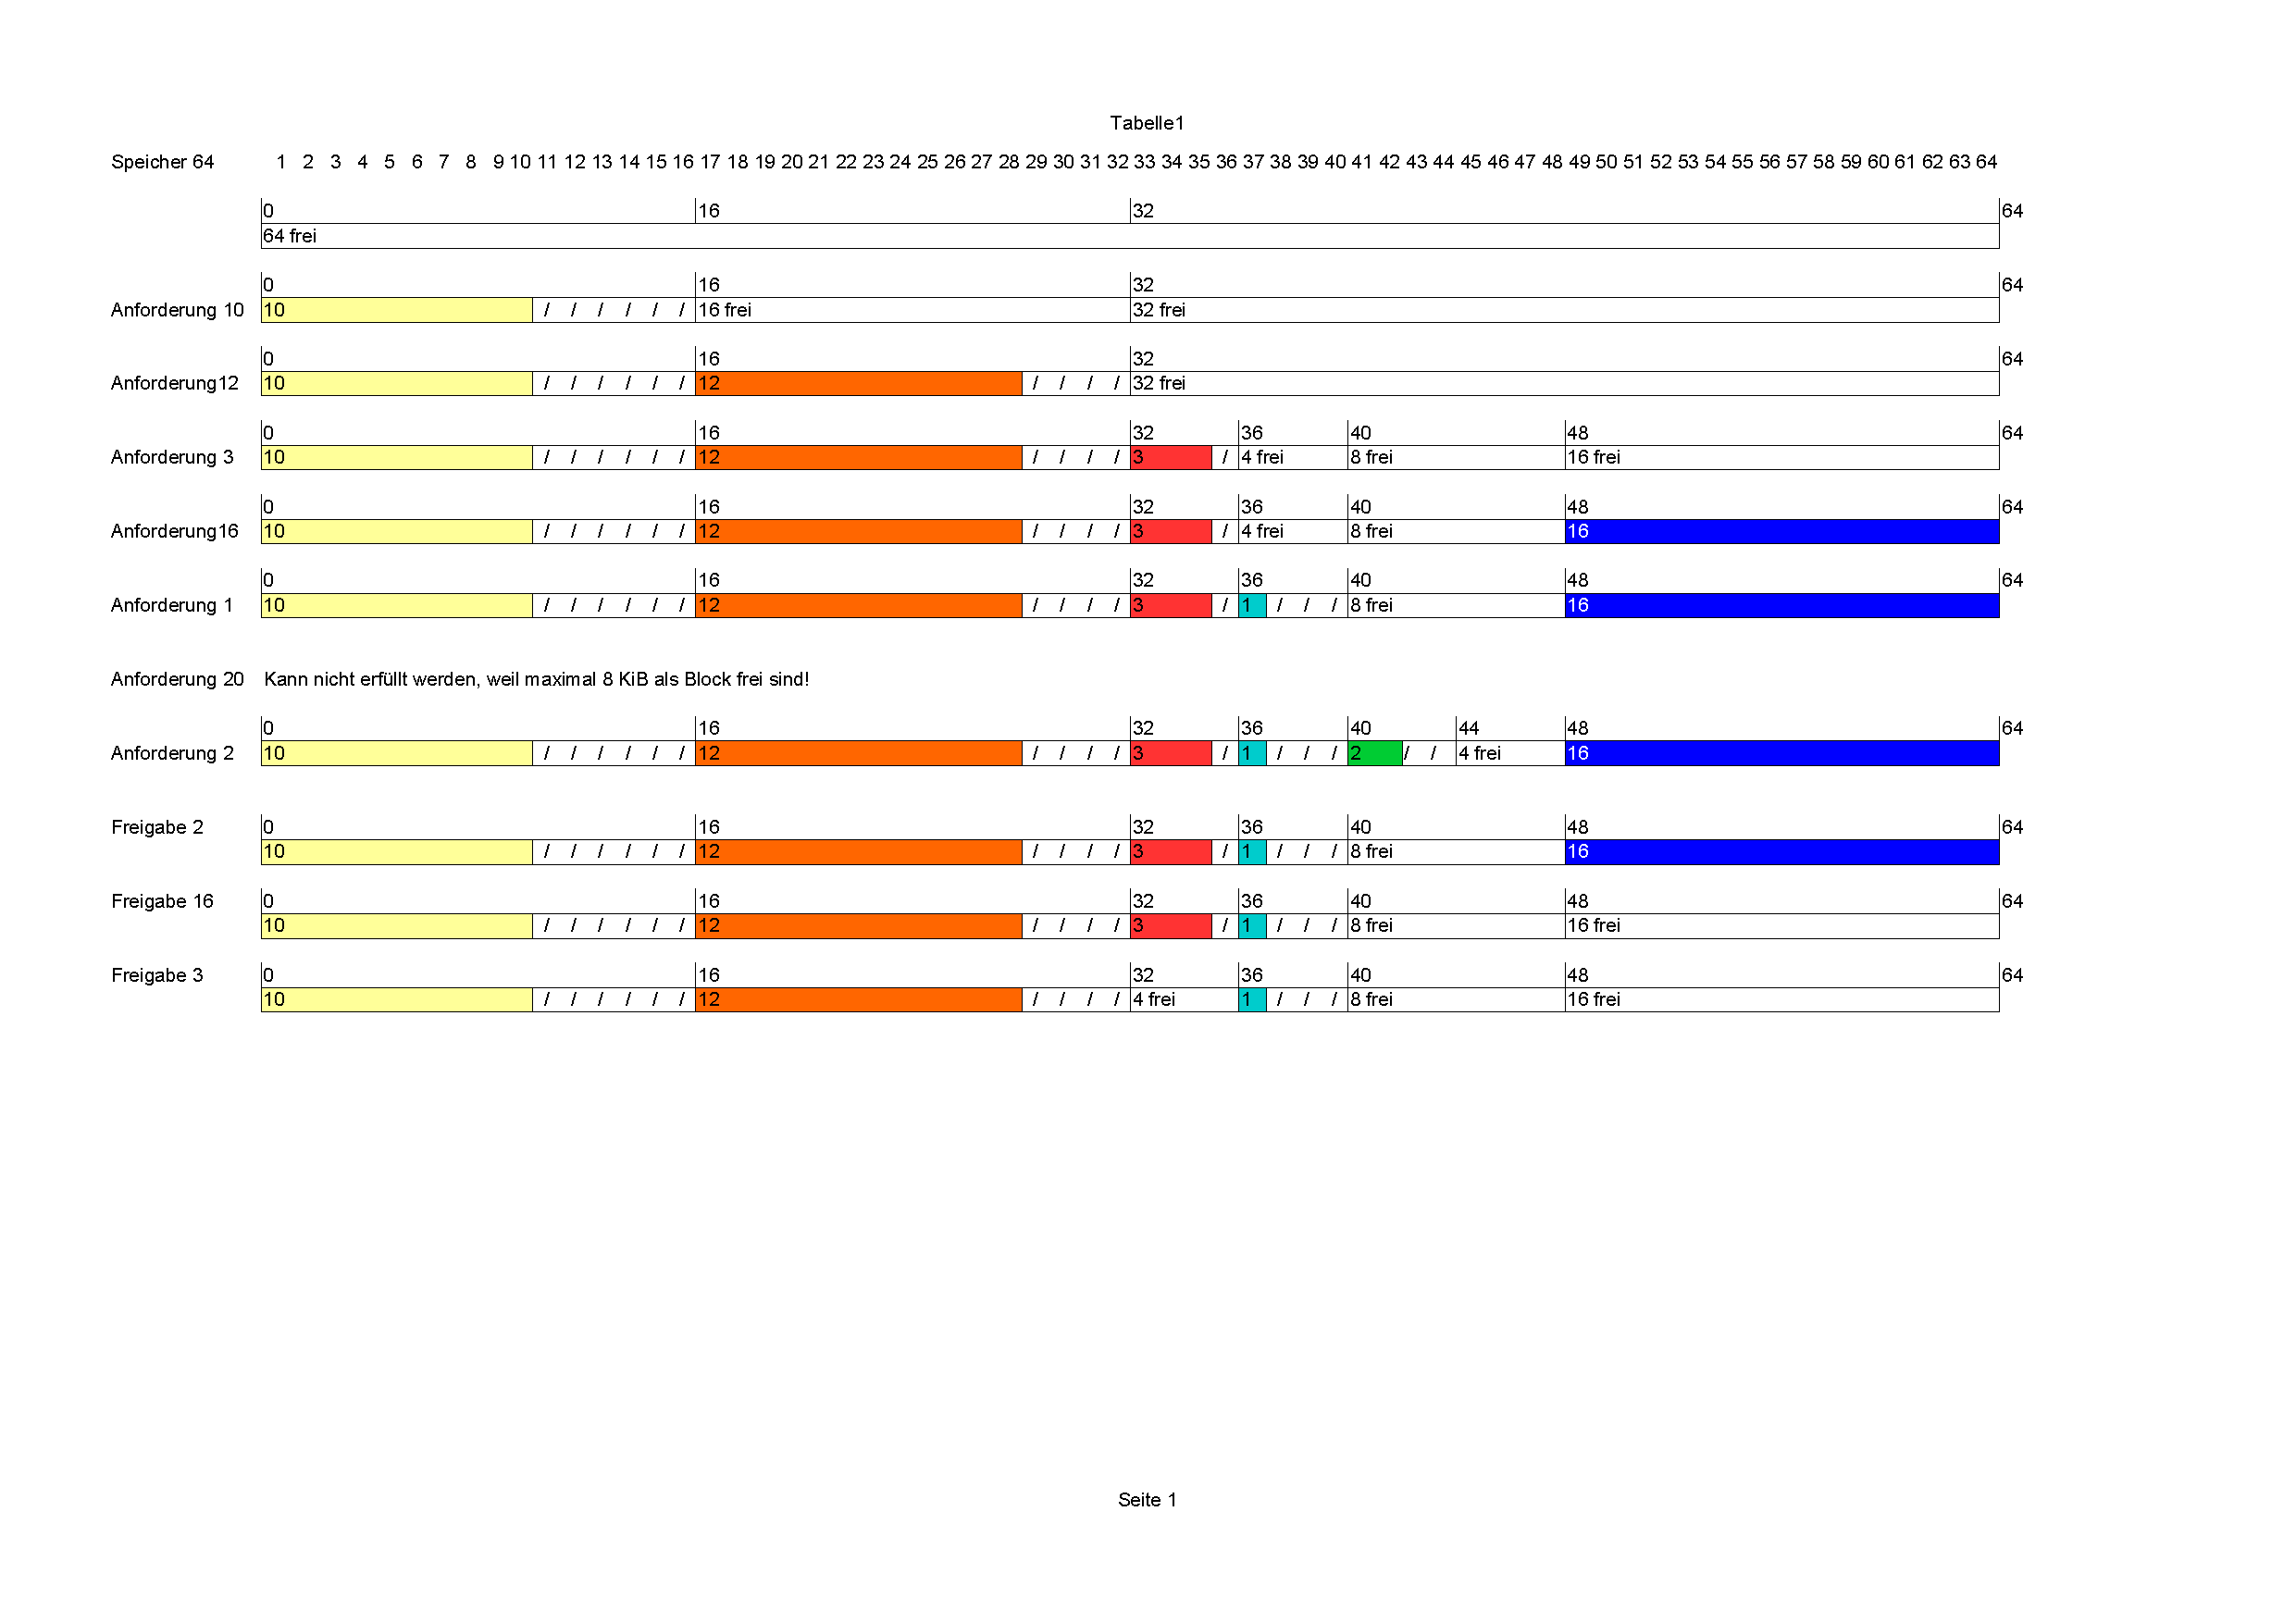
\includegraphics[width=1.25\textwidth]{Aufgabe_2.pdf}
\end{figure}
\clearpage
\section*{Aufgabe 3}
\begin{figure}[h]
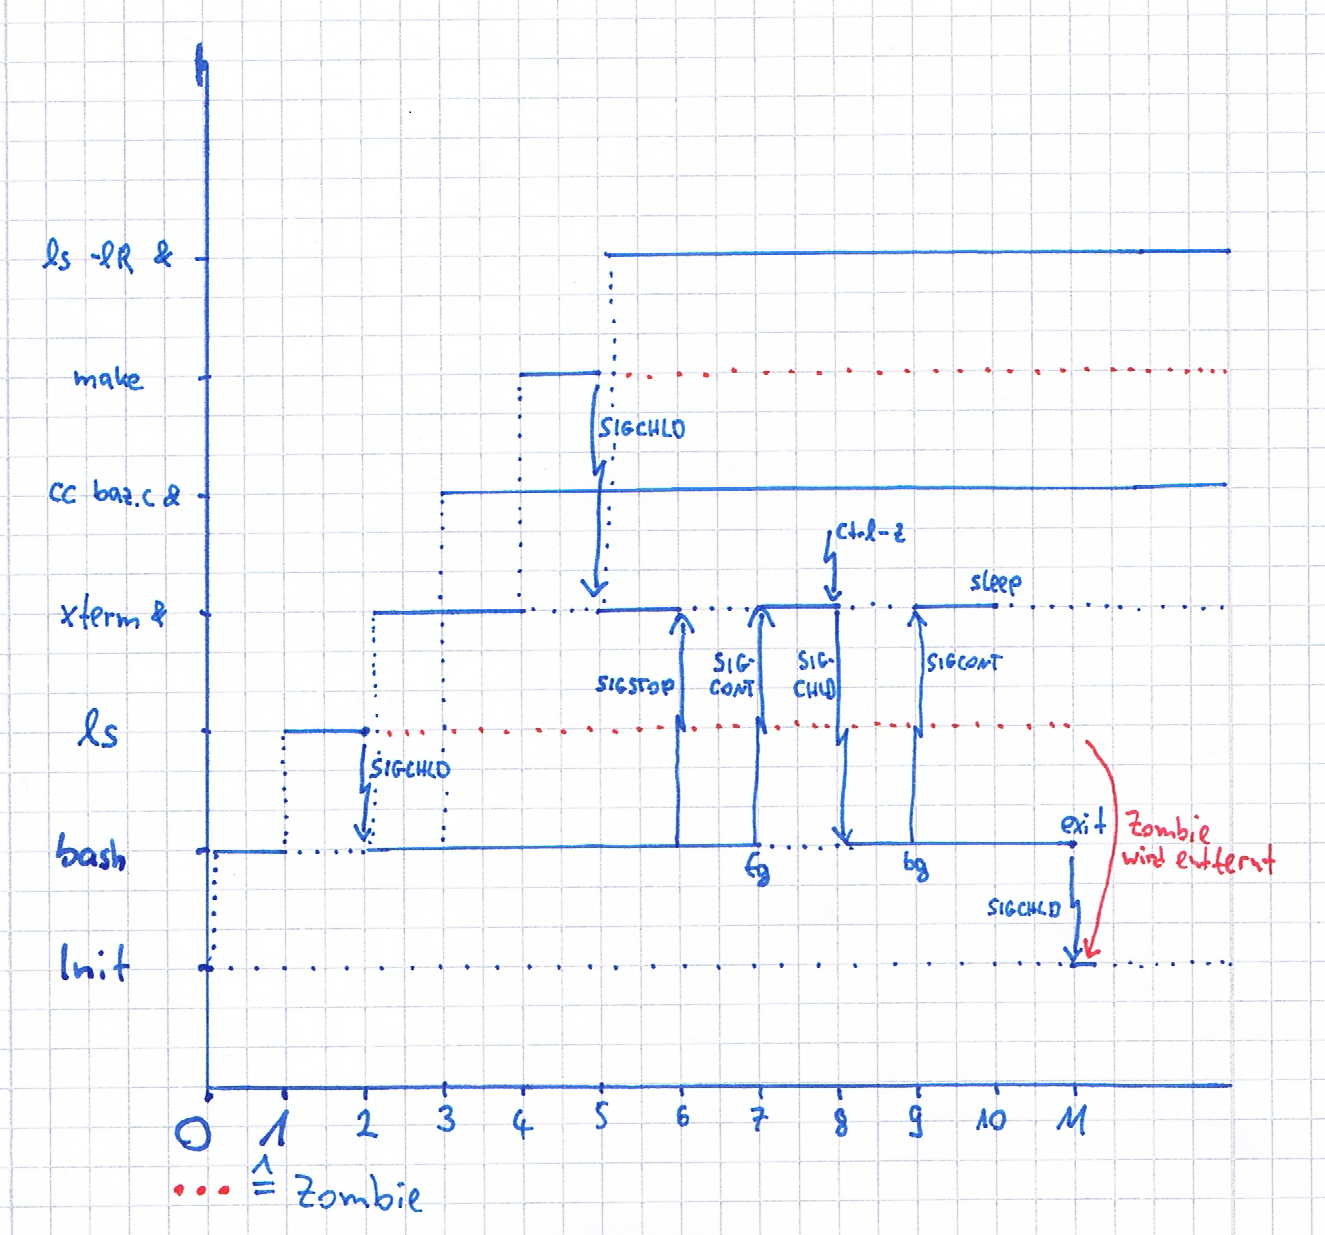
\includegraphics[width=1.1\textwidth]{pic.png}
\end{figure}
Das gestartete Terminal m"usste nun zu \emph{Init} geh"oren, da der urspr"ungliche Elternprozess \emph{bash} terminiert ist.
\end{document}
